%%%%%%%%%%%%%%%%%%%%%%%%%%%%%%%%%%%%%%%%%%%%%%%%%%%%%%%%%%%%%%%%%%%%%%%%
% Plantilla TFG/TFM
% Escuela Politécnica Superior de la Universidad de Alicante
% Realizado por: Jose Manuel Requena Plens
% Contacto: info@jmrplens.com / Telegram:@jmrplens
%%%%%%%%%%%%%%%%%%%%%%%%%%%%%%%%%%%%%%%%%%%%%%%%%%%%%%%%%%%%%%%%%%%%%%%%

\chapter{Desarrollo}
\label{desarrollo}

\section{Expanding the UnrealROX Framework}
As we previously mentioned on section \ref{introduction} one of the main goals on this work is to expand the UnrealROX framework to easily generate synthetic data. In this section we will further detail UnrealROX framework and the data generation process.

UnrealROX can automatically generate and annotate data from a recorded sequence, but manually recording can be tedious and time consuming. In this work we have built the basic framework for the programmer to include its own actions and execute them in a sequential way, much like other frameworks like VirtualHome \cite{virtualhome2018}. 

\subsection{The ROXBasePawn Class}
This is the main class that contains all the logic for the character controller (movement, animations, grasping) of any robot pawn. It allows for the user introduce a robot to the scene and manually move and interact with the objects in a scene.

\subsection{The ROXBotPawn Class}
The ROXBotPawn class inherits from ROXBasePawn and will handle all the logic for the automation of tasks of any \textit{Pawn} within a scene. In order to model all the different actions and interactions the Enum $EActionType$ was created, here the programmer can add any type of action to be built into the system.

Also in order to model the actions themselves, the $FROXAction$ struct was built, containing a pointer to the target, as well as the type of action $EActionType$, the structure is shown in listing \ref{code:actionStruct}.

\begin{listing}[language=C++, caption=FROXAction struct, frame=single, label=code:actionStruct]
	USTRUCT(BlueprintType)
	struct FROXAction
	{
		GENERATED_USTRUCT_BODY()
		UPROPERTY(BlueprintReadWrite, EditAnywhere, Category = Pathfinding)
		AActor* target;
		
		UPROPERTY(BlueprintReadWrite, EditAnywhere, Category = Pathfinding)
		EActionType action;
		
		FROXAction() : target(nullptr), action(EActionType::MoveTo) {};
		FROXAction(AActor* tg, EActionType t) : target(tg), action(t) {};
	}
\end{listing}

In order for the programmer to add actions and queue them from the \gls{ue4} editor we built the $doAction(AActor*, EActionType)$ and made it BlueprintCallable, this way, in a simple way actions can be queued from the editor and the $Pawn$ will execute them in a sequential order as seen in figure \ref{action_queue}.

\begin{figure}[h]
	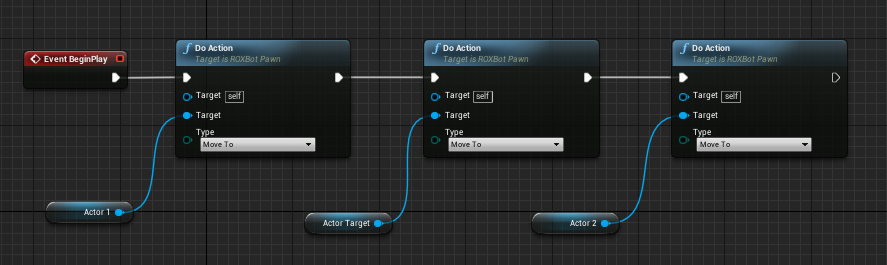
\includegraphics[scale=0.4]{archivos/action_queue.png}
	\centering
	\caption{Example of queuing 3 "MoveTo" actions from the editor}
	\label{action_queue}
\end{figure}

The $doAction()$ method creates a $FROXActions$ and pushes it to the queue. Whenever the queue contains an action and the $Pawn$ is not executing one, it will run the $fetchNextAction()$ method. This will pop the action from the queue and execute the method corresponding to that action.

\todo{EQS and Naive MoveToActor methods of the UE4 Character class}


Additionally, pathfinding and movement logic was implemented in order to define the $MoveTo$ action. In a first approach, the MoveTo method of the  For this purpose the NavigationMesh component of \gls{ue4} was used along with the $FindPathToActorSynchronously$ method, which returns a $UNavigationPath$ containing all the path-points from one actor to another. Once we obtain the pathpoints the $VInterpConstantTo$ from the FMath library and the $RInterpTo_Constant$ from the UKismeMathLibrary are used in order to obtain the next vector transformation for both position and rotation of the $Pawn$, this movemement logic can be seen in listing \ref{code:movementLogic}. These methods interpolate the current location with the next path-point location in order to achieve a smooth transition and make the movement more natural.

\begin{listing}[language=C++, caption=Movement logic for the pathfinding algorithm, frame=single, label=code:movementLogic]
	FVector nextPos = FMath::VInterpConstantTo(this->ActorLocation(), FVector(pathPoints[i].X, pathPoints[i].Y, ActorLocation().Z), DeltaTime, vel);
	FRotator nextRot = UKismetMathLibrary::RInterpTo_Constant(ActorRotation(), UKismetMathLibrary::FindLookAtRotation(ActorLocation(), nextPos), DeltaTime, rotateVel);
	SetActorRotation(nextRot);
	SetActorLocation(nextPos);
\end{listing}